\documentclass[12pt,]{article}


\usepackage{baskervillef}%polskie znaki może nie

%flow chatry
\usepackage{tikz}
\usetikzlibrary{shapes.geometric, arrows}
\usepackage{amssymb}
\usepackage{float}

\title{Sprawozadanie lernicng}
\author{Tymon Łazowy}
\date{123,2123,12}


\tikzstyle{startstop} = [ellipse, rounded corners, minimum width=2cm, minimum height=1cm,text centered, draw=black,thick,fill=red!0]

\tikzstyle{io} = [trapezium,
trapezium stretches=true,
trapezium left angle=70,
trapezium right angle=110,
thick,minimum width=2cm,
minimum height=0.85cm,
text centered,
draw=black,
fill=blue!0]

\tikzstyle{process} = [rectangle,minimum height=0.85cm,text centered,draw=black,thick,]

\tikzstyle{decision} = [diamond,minimum width=1cm, minimum height=1cm, text centered, draw=black, fill=green!0,thick]

\tikzstyle{arrow} = [thick,->,>=stealth]

\begin{document}
D: a,b,c liczby $\in \mathbb{N}_0$

S: max najwieksza liczba $\in \mathbb{N}_0$ 
\begin{figure}[h]
   
    \caption{1.11 flowchart} 
    \centering  
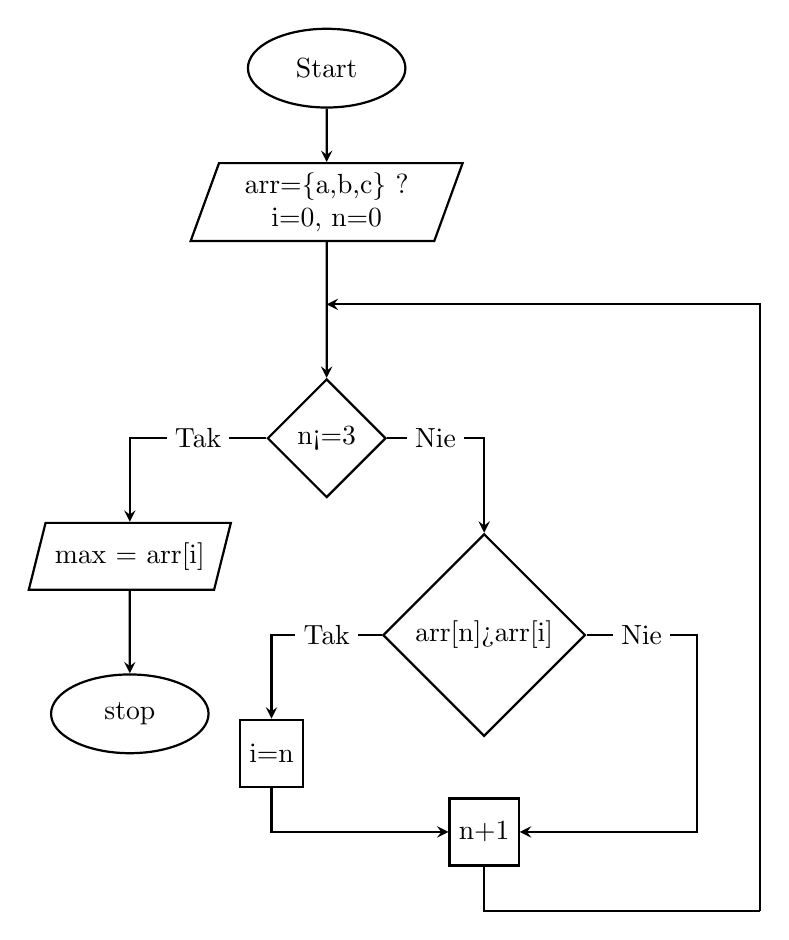
\begin{tikzpicture}[node distance=1.5cm]

\node (start) [startstop] {Start};
\node (in1) [io, below of=start,text width=2.5cm, yshift=-0.2cm] {arr=\{a,b,c\} ?

i=0, n=0};
\node (dec1) [decision, below of=in1, yshift=-1.5cm] {n<=3};
\node (tak1) [io, left of=dec1, xshift=-1cm, yshift=-1.5cm] {max = arr[i]};
\node (stop) [startstop, below of =tak1,yshift=-0.5cm]{stop};
\node (nie1) [decision, right of=dec1, xshift=0.50cm, yshift=-2.5cm] {arr[n]>arr[i]};
\node (tak2) [rectangle,minimum height=0.85cm,text centered,draw=black,thick,left of=nie1,xshift=-1.2cm, yshift=-1.5cm,] {i=n};
\node (nie2) [coordinate, right of=nie1,xshift=1.2cm,yshift=-2cm]{};
\node (pro2) [rectangle,minimum height=0.85cm,text centered,draw=black,thick,below of=nie1, yshift=-1cm] {n+1};
\node (meet) [coordinate, below of=in1,yshift=0.2cm]{};
\node (meet2) [coordinate, right of=pro2,xshift=2cm,yshift=-1cm]{};

\draw [arrow] (start) -- (in1);
\draw [arrow] (in1) -- (dec1);
\draw[arrow] (dec1) -| (tak1) node[pos=0.25,fill=white,inner sep=3]{Tak};
\draw[arrow] (dec1) -| (nie1) node[pos=0.25,fill=white,inner sep=3]{Nie};
\draw[arrow] (nie1) -| (tak2) node[pos=0.25,fill=white,inner sep=3]{Tak};
\draw[thick] (nie1) -| (nie2) node[pos=0.25,fill=white,inner sep=3]{Nie};   
\draw [arrow] (nie2) |- (pro2);
\draw [arrow] (tak2) |- (pro2);
\draw [thick] (pro2) |- (meet2);
\draw [arrow] (meet2) |- (meet);
\draw [arrow] (tak1)--(stop);



\end{tikzpicture}
    
    \label{flow11}
\end{figure}
\end{document}